% Architecture of U-net
% Author: zhyantao
\documentclass[border=10pt]{standalone}

\usepackage{verbatim}
\usepackage{tikz}
\usetikzlibrary{arrows.meta}
\tikzset{%
  >={Latex[width=2mm,length=2mm]},
  % Specifications for style of nodes:
            base/.style = {rectangle, rounded corners, draw=black,
                           minimum width=4cm, minimum height=1cm,
                           text centered, font=\sffamily},
  activityStarts/.style = {base, fill=blue!30},
       startstop/.style = {base, fill=red!30},
   max_pooling2d/.style = {base, fill=green!30},
     up_sampling/.style = {base, fill=green!30},
         process/.style = {base, minimum width=2.5cm, fill=orange!15,
                           font=\ttfamily},
}
\begin{document}    
% Drawing part, node distance is 1.5 cm and every node
% is prefilled with white background
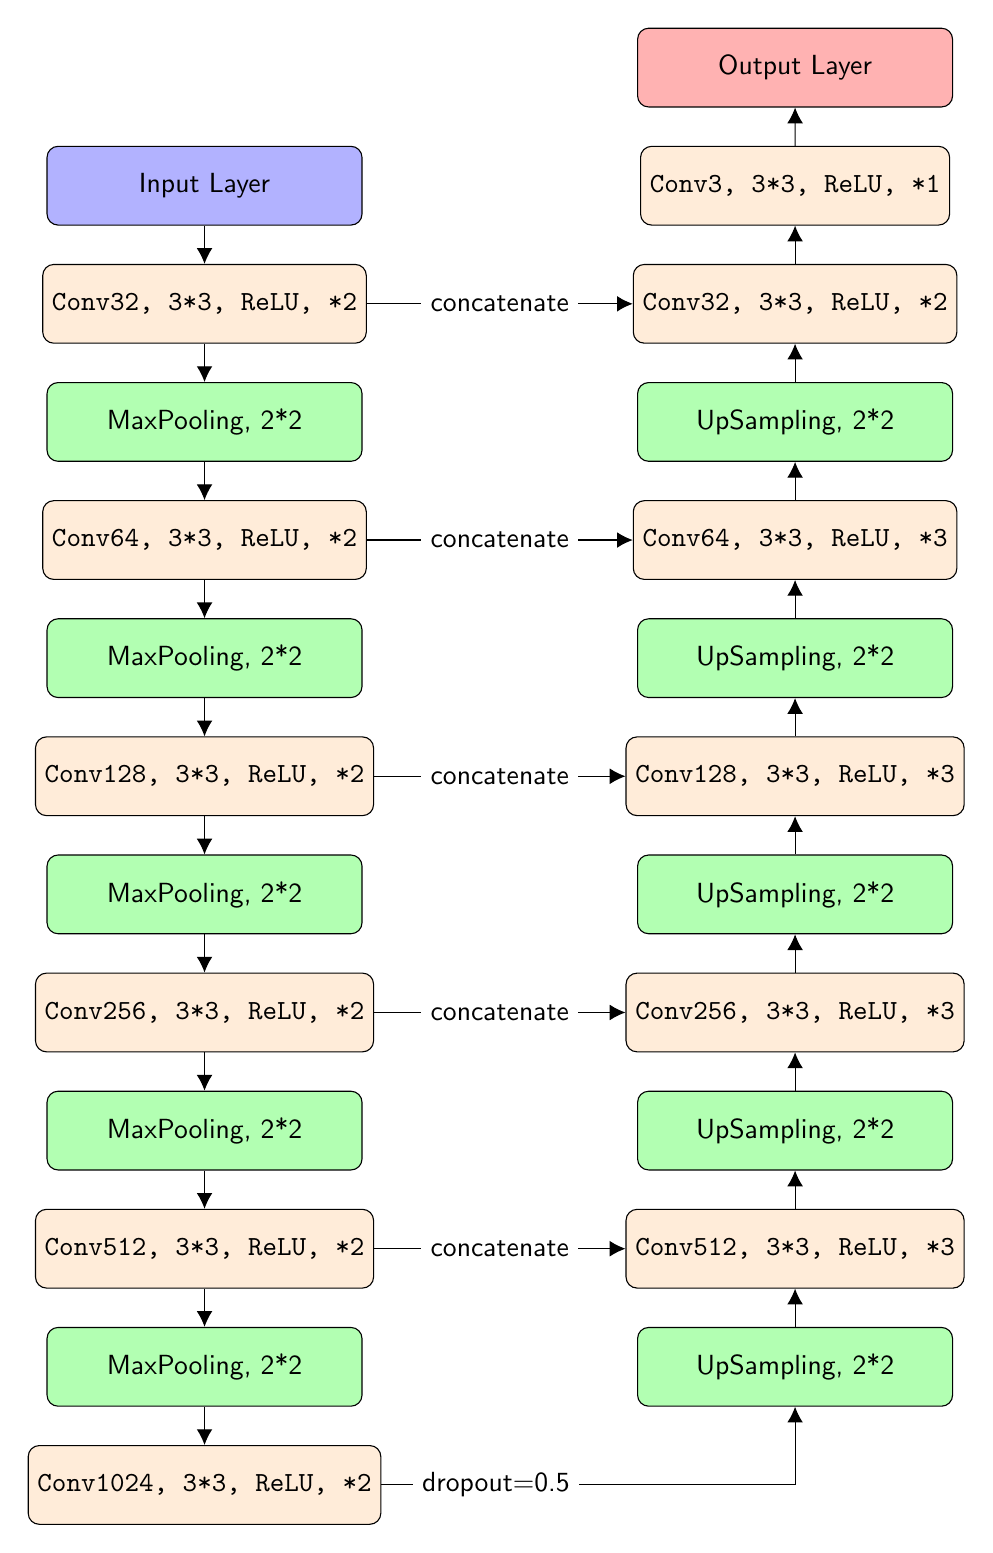
\begin{tikzpicture}[node distance=1.5cm,
    every node/.style={fill=white, font=\sffamily}, align=center]
  % Specification of nodes (position, etc.)
  \node (inputLayer)          [activityStarts]							{Input Layer};
  
  \node (conv2d_1)            [process, below of=inputLayer]			{Conv32, 3*3, ReLU, *2};
  \node (max_pooling2d_1)     [max_pooling2d, below of=conv2d_1]		{MaxPooling, 2*2};
  
  \node (conv2d_3)            [process, below of=max_pooling2d_1]		{Conv64, 3*3, ReLU, *2};
  \node (max_pooling2d_2)     [max_pooling2d, below of=conv2d_3]		{MaxPooling, 2*2};
  
  \node (conv2d_5)            [process, below of=max_pooling2d_2]		{Conv128, 3*3, ReLU, *2};
  \node (max_pooling2d_3)     [max_pooling2d, below of=conv2d_5]		{MaxPooling, 2*2};
  
  \node (conv2d_7)            [process, below of=max_pooling2d_3]		{Conv256, 3*3, ReLU, *2};
  \node (max_pooling2d_4)     [max_pooling2d, below of=conv2d_7]		{MaxPooling, 2*2};
  
  \node (conv2d_9)            [process, below of=max_pooling2d_4]		{Conv512, 3*3, ReLU, *2};
  \node (max_pooling2d_5)     [max_pooling2d, below of=conv2d_9]		{MaxPooling, 2*2};
  
  \node (conv2d_11)           [process, below of=max_pooling2d_5]		{Conv1024, 3*3, ReLU, *2};
  
  \node (upsampling_1)        [up_sampling, right of=max_pooling2d_5, xshift=6cm] 	{UpSampling, 2*2};
  \node (conv2d_13)           [process, right of=conv2d_9, xshift=6cm]      		{Conv512, 3*3, ReLU, *3};
  
  \node (upsampling_2)        [up_sampling, right of=max_pooling2d_4, xshift=6cm]  	{UpSampling, 2*2};
  \node (conv2d_16)           [process, right of=conv2d_7, xshift=6cm]				{Conv256, 3*3, ReLU, *3};
  
  \node (upsampling_3)        [up_sampling, right of=max_pooling2d_3, xshift=6cm]	{UpSampling, 2*2};
  \node (conv2d_19)           [process, right of=conv2d_5, xshift=6cm]      		{Conv128, 3*3, ReLU, *3};
  
  \node (upsampling_4)        [up_sampling, right of=max_pooling2d_2, xshift=6cm]  	{UpSampling, 2*2};
  \node (conv2d_22)           [process, right of=conv2d_3, xshift=6cm]      		{Conv64, 3*3, ReLU, *3};
  
  \node (upsampling_5)        [up_sampling, right of=max_pooling2d_1, xshift=6cm]	{UpSampling, 2*2};
  \node (conv2d_25)           [process, right of=conv2d_1, xshift=6cm]    			{Conv32, 3*3, ReLU, *2};
  \node (conv2d_29)           [process, right of=inputLayer, xshift=6cm]    		{Conv3, 3*3, ReLU, *1};

  \node (outputLayer)         [startstop, xshift=7.5cm, yshift=1.5cm]  				{Output Layer};
   
  % Specification of lines between nodes specified above
  % with aditional nodes for description 
  \draw[->]          (inputLayer) -- (conv2d_1);
  \draw[->]     	   (conv2d_1) -- (max_pooling2d_1);
  \draw[->]     (max_pooling2d_1) -- (conv2d_3);
  \draw[->]            (conv2d_3) -- (max_pooling2d_2);
  \draw[->]     (max_pooling2d_2) -- (conv2d_5);
  \draw[->]            (conv2d_5) -- (max_pooling2d_3);
  \draw[->]     (max_pooling2d_3) -- (conv2d_7); 
  \draw[->]            (conv2d_7) -- (max_pooling2d_4);
  \draw[->]     (max_pooling2d_4) -- (conv2d_9);
  \draw[->]            (conv2d_9) -- (max_pooling2d_5);
  \draw[->]     (max_pooling2d_5) -- (conv2d_11);
  
  \draw[->]           (conv2d_11) -| node [xshift=-3.8cm] {dropout=0.5} (upsampling_1);
  \draw[->]		   (upsampling_1) -- (conv2d_13);
  \draw[->]		   	  (conv2d_13) -- (upsampling_2);
  \draw[->]		   (upsampling_2) -- (conv2d_16);
  \draw[->]		      (conv2d_16) -- (upsampling_3);
  \draw[->]		   (upsampling_3) -- (conv2d_19);
  \draw[->]		      (conv2d_19) -- (upsampling_4);
  \draw[->]		   (upsampling_4) -- (conv2d_22);
  \draw[->]		      (conv2d_22) -- (upsampling_5);
  \draw[->]		   (upsampling_5) -- (conv2d_25);
  \draw[->]		      (conv2d_25) -- (conv2d_29);
  \draw[->]		      (conv2d_29) -- (outputLayer);
  
  \draw[->]		       (conv2d_1) -- node {concatenate} (conv2d_25);
  \draw[->]		       (conv2d_3) -- node {concatenate} (conv2d_22);
  \draw[->]		       (conv2d_5) -- node {concatenate} (conv2d_19);
  \draw[->]		       (conv2d_7) -- node {concatenate} (conv2d_16);
  \draw[->]		       (conv2d_9) -- node {concatenate} (conv2d_13);

  \end{tikzpicture}
\end{document}